% Created 2022-09-19 Mon 22:00
\documentclass[9pt, b5paper]{article}
\usepackage{xeCJK}
\usepackage{minted}
\usepackage[T1]{fontenc}
\usepackage[scaled]{beraserif}
\usepackage[scaled]{berasans}
\usepackage[scaled]{beramono}
\usepackage{graphicx}
\usepackage{xcolor}
\usepackage{multirow}
\usepackage{multicol}
\usepackage{float}
\usepackage{textcomp}
\usepackage{algorithm}
\usepackage{algorithmic}
\usepackage{latexsym}
\usepackage{natbib}
\usepackage{geometry}
\geometry{left=1.2cm,right=1.2cm,top=1.5cm,bottom=1.2cm}
\newminted{common-lisp}{fontsize=\footnotesize} 
\usepackage[xetex,colorlinks=true,CJKbookmarks=true,linkcolor=blue,urlcolor=blue,menucolor=blue]{hyperref}
\author{Heyan Jenny Huang}
\date{\today}
\title{Appellant's Desigtnation of Record on Appeal}
\hypersetup{
  pdfkeywords={},
  pdfsubject={},
  pdfcreator={Emacs 27.1 (Org mode 8.2.7c)}}
\begin{document}

\maketitle
\tableofcontents


\section{Other court cases}
\label{sec-1}

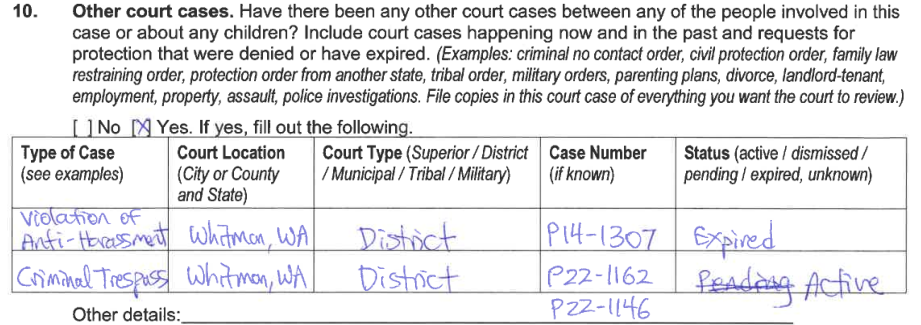
\includegraphics[width=.9\linewidth]{./pic/dearCousin_20220919_153339.png}
\subsection{There are 2 ACTIVE cases going on: \textbf{P22-1146} and \textbf{P22-1162};}
\label{sec-1-1}
\subsubsection{\textbf{P22-1146:}}
\label{sec-1-1-1}

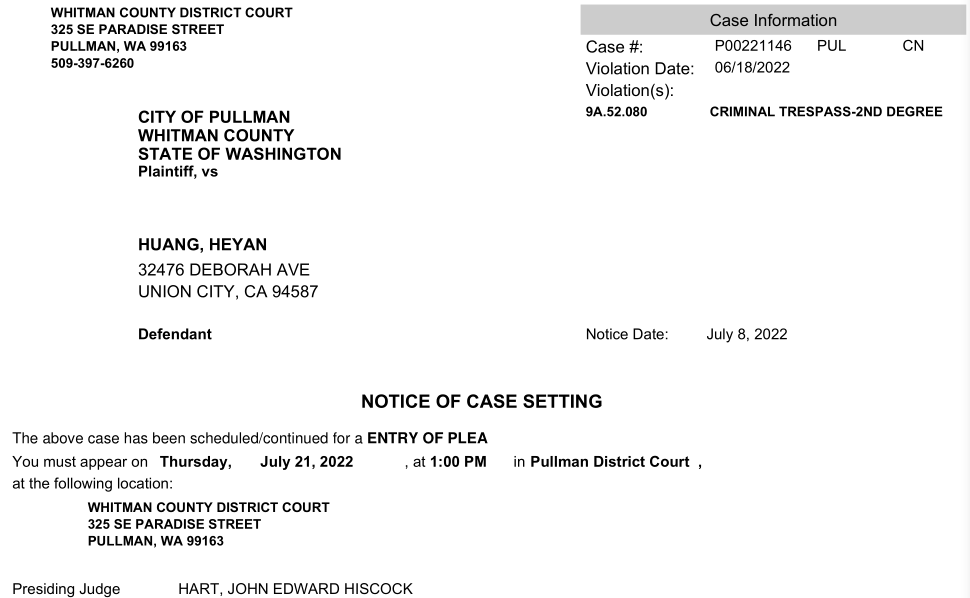
\includegraphics[width=.9\linewidth]{./pic/dearCousin_20220919_185022.png}
\begin{itemize}
\item Due to the slightly relatively late response of court arrangement of hearing, a person without necessary boundary understandings does NOT have the necessary chance in time to learn and self-correct his/her behavior after ONE such mistake.
\end{itemize}
\subsubsection{\textbf{P22-1162:}}
\label{sec-1-1-2}

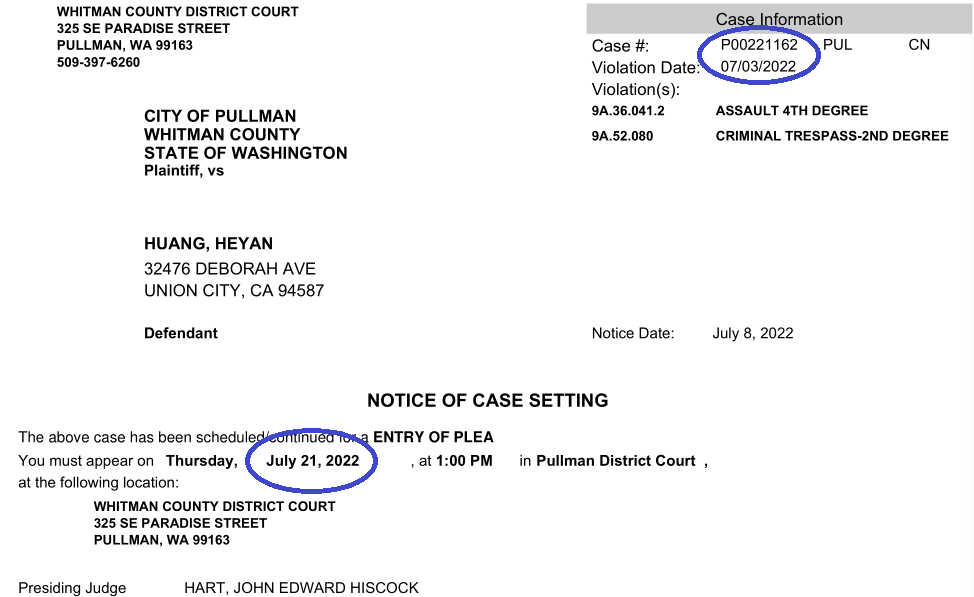
\includegraphics[width=.9\linewidth]{./pic/dearCousin_20220919_185057.png}
\begin{itemize}
\item There are 2 Active cases, but the cases were only taken care of after the second P22-1162 incident, \textbf{which date for both cases were set up hearing on July 21, 2022}, and which were after the 2nd incident and I would have NO chance/opportunity to learn nor correct myself without IN TIME hearing after 1st incident.
\end{itemize}
\subsubsection{There is 1 EXPIRED case of \textbf{P14-1307}}
\label{sec-1-1-3}
\begin{itemize}
\item 是当地的法院没有及时地通知我或是办理案件,让我没有机会学习和校正自己的行为, 不管是6/17号的,还是接下来的,我没有机会学习来校正自己
\end{itemize}

\section{Length of Order一年,多于一年,一辈子(法官真是生猛呀,一令就是一辈子。。。。。)}
\label{sec-2}

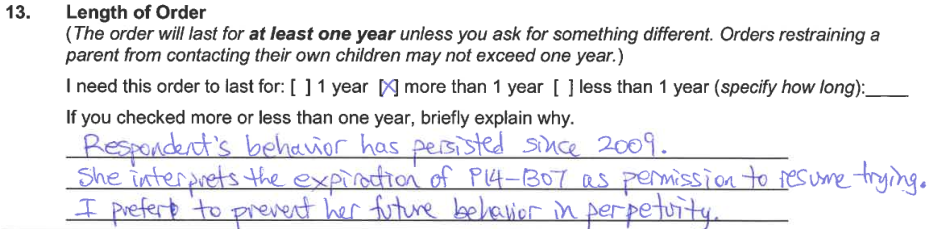
\includegraphics[width=.9\linewidth]{./pic/dearCousin_20220919_153711.png}
\begin{itemize}
\item Who came to US as an international student, \textbf{I do NOT have nor by any means learn and understand these legal terms}, and I \textbf{DO have been} interpreting the expireation of P14-1307 as permission to resume trying. As an previous girl friend who is still deeply falling in love for a previous boyfriend, who will stop trying by any means though?
\item We understand petitioner's understandable intention, but \textbf{we also need to consider and allow the respnodent chance and opprotunities to grow, to learn as well as correct herself}, instead of setting up permanent protection orders without reasonable consideration on response's side of story and feelings.
\item 是的,我以为保护令的期限到了便是过期了,我便可以retry 恢复男女朋友关系了。。。
\item 听证会上,我向法官陈述了,我是国际留学生,对美国社会法律并不了解;
\end{itemize}

\section{Most Recent Incident}
\label{sec-3}

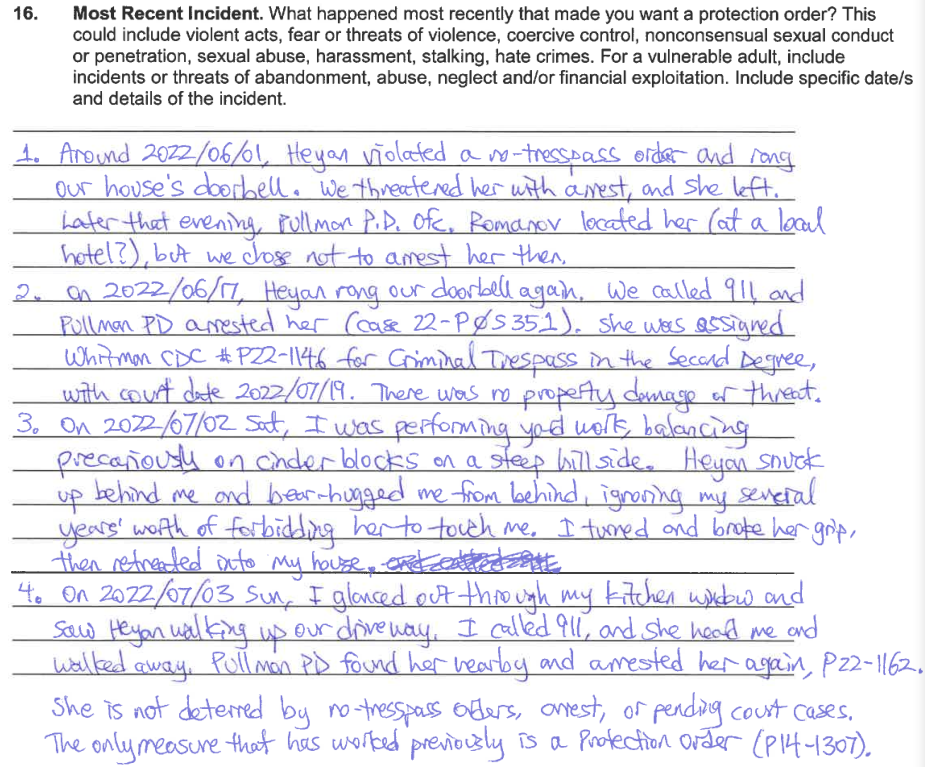
\includegraphics[width=.9\linewidth]{./pic/dearCousin_20220919_183412.png}
\begin{itemize}
\item Your honor, my explaination are as following listed:
\item 1. I \textbf{did have interpreted expired protection orders as permission of allowance for retrying}. And it had been the reason that I had been visited back during 2021 upon which year I devorced ex-husband, and want to retry the relationship with Mr. Eric Shing-suan Wang. And I did have visted quite a few times back then, \emph{\textbf{2 times last year in 2021}}, in end of \textbf{March 2021}, \textbf{July 30th, 2021}, and followed with \emph{\textbf{3 times visitings this years in}} \textbf{end of May}, \textbf{middle of June}, as well as \textbf{beginning of July.}
\item 1. \emph{\textbf{There was a policement did call me when I was about to register for a hotel room in end of May 2022}}, but \textbf{the unreasonable expiring date of 2099 the policeman warned me over the phone} made me believe that \textbf{it was more a threatens from a unprofessional small town policeman, which cases had happened on me before, on 12/27/2014 I had been arrested by unprofessional small town policeman who had absolutely no right to arrest me at that time, but he did.}
\item 2. I \textbf{was arrested by the policeman on 6/17/2022}. But I was raised up in a large family together with 3 elder siblings from a farm of an undeveloped coutry, and \textbf{I had NOT been taken good care of during my childhood}, and \textbf{am grown up with to some extend disability of missing concepts of boundaries}. I knew that Mr. Eric Shing-suan Wang had warned me on NOT going to the house, but back then I was NOT able to understand how serious the warn could be. And even at my ago in my early forties, I am still practicing various boundaries during my daily life. Personally I need court's hearing's help, judge's help to help behavior correct me and help me set up boundaries as well as help me understand how important and severe things could potentially be.
\item 3. Your honor, it was one of the afternoon that I have driven more than 1000 miles one way within less than 24 hours, and I was tired, only saw a person in between the two neighbourhood houses. As an international student, I don't have any concepts that I am NOT allowed to enter any household's backyard, not only Mr. Eric Shing-suan Wang's, and \textbf{it was in between open yards of two neighbourhood houses without any marks/WARNING stating NO ENTERING}, i was just trying to get close to see backyeard scene, but \textbf{due to the steep hillside and my tiredness, I run out of balance, and to prevent myself from hitting onto hard steep hillside stones, I ended of snuck a person nearby, which turned out to be Mr. Eric Shing-suan Wang} who i was warned NOT to touch, but it was completely a situation of tired person out of balance. Your honor, please help understand the tiredness of driving more than 1000 miles continuously within less than 24 hours. Thanks for your understanding so much!
\item 4. Your honor, \textbf{I was NOT intended to, and I had even driven more than 20 miles on my way back to CA, and I had even grabbed groceries (water) from neighbouring town} (Please check below receipt \textbf{form neighbouring town Colfax, WA} before the backed to Pullman arrestment). But due to the heavy rain which I had waited the whole day before I left for home that day, \textbf{experiencing the heavy rain on my way to Colfax, I decided to drive back to visit WSU campus after the raining when the campus was wet}. When I driving by the house, I saw windows were all closed, and mis-signally resulted in an unwanted driveway walk. And that's all.
\end{itemize}

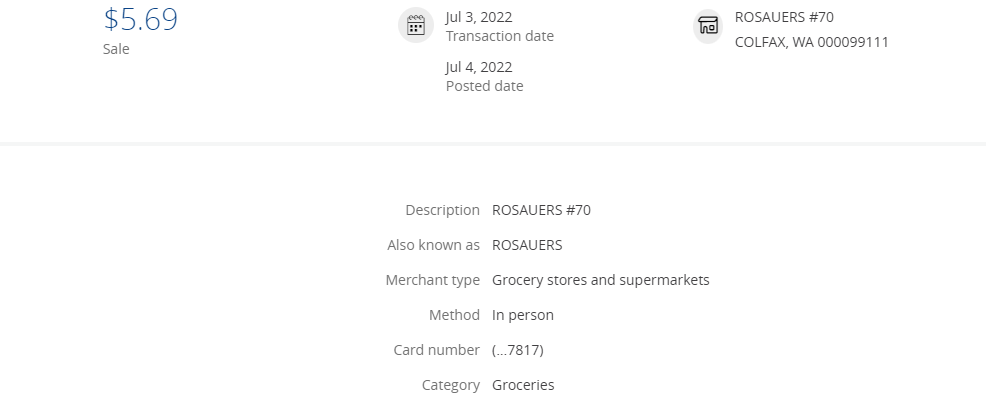
\includegraphics[width=.9\linewidth]{./pic/dearCousin_20220919_201117.png}
\section{Past Incidents}
\label{sec-4}

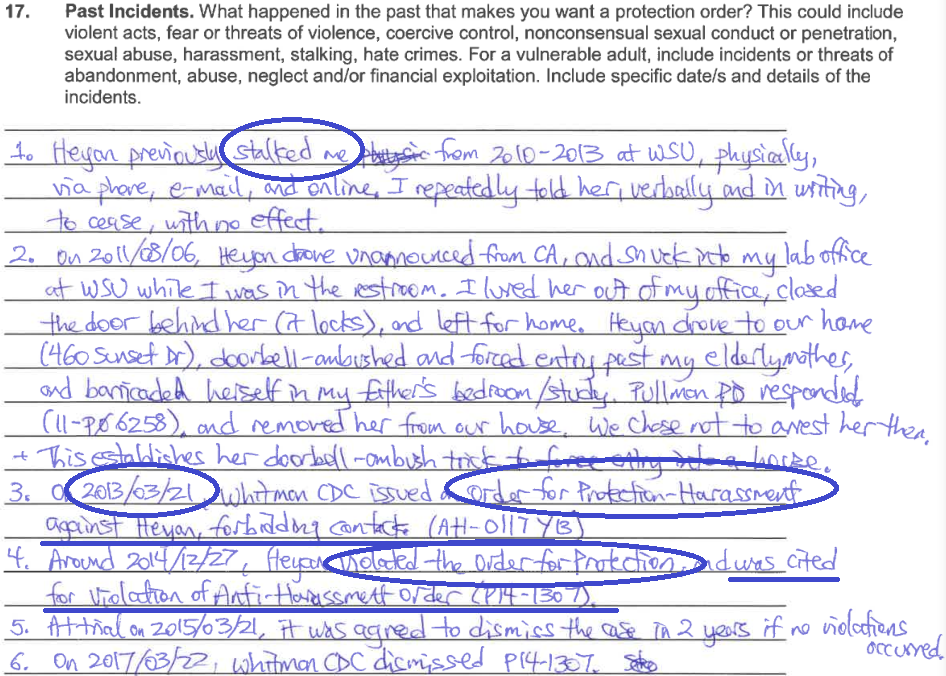
\includegraphics[width=.9\linewidth]{./pic/dearCousin_20220919_183625.png}
\begin{itemize}
\item Your honor, my explaination are as following listed:
\item 1. Your honor, back between 2010-2013, I was only in my early thirties. For others must be an age of mature enough, but for me personally, I was still naive, and with the missing boundaries concepts and understandings, I was sincerely NOT able to understand and digest what had been going on during those ages.
\item 2. Your honor, what was stated was completely correct, but at that age I was NOT able to understand what's going on, nor be able to reasonably understand the relationships.
\item 3. \textbf{Case No. AH-0117YB ORDER FOR PROTECTION HARASSMENT was a completely mis-manipulated case executed upon me -- a naive international student}. 
\begin{itemize}
\item I have \textbf{NOT been notified any hearing for this Harassment protection order against me, nor had been served the protection order when it was effiective.}
\item I \textbf{was only able to get a copy on 12/29/2014 upon which day I had been arrested for this order}, and upon when I have NO idea about any protection order against me, only that the police who arrested me mentioned once that I could ask for the file when I were able to be bonded out of the jail on 12/29/2014.
\item \textbf{The protection order was finally served to me on court date 2/27/2015.} But it had put me into all kinds of psychological problems the whole spring 2015 during my naive age when I was NOT able to digest the whole case and all the threatening it brought into my life.
\item And \textbf{the protection order against me during my naive age eventually resulted in a mistaken unthoughtful marriage which I regret all the time and would wish I had never got maried once when I was NOT being able to digest the protection whole 4-year length protection order against me.}
\end{itemize}
\item 4. I did visit Mr. Eric Shing-suan Wang's office on 12/27/2014. And got arrested that day. But your honor, please help learn the facts stated above also that: 
\begin{itemize}
\item \textbf{I had NEVER been notified any protection order hearing, nor had been served any protection order file, and I had NO concepts NO impression about any protection order before 12/27/2014.}
\item My last case back then of \textbf{PC011713 was settled down on 3/7/2013, and the case would dismiss on 3/7/2014.}
\item As \textbf{an naive international student who was NOT able to digest the legal terms nor got enough help}, and I \textbf{did interpret it as after 3/7/2014, I would be permitted to retry. And I wainted half more year till 12/27/2014 to retry and revisit Mr. Eric Shing-suan Wang's student office.} And I got arresteded.
\end{itemize}
\item 5. \textbf{I was formally served the protection order AH-0117YB ORDER FOR PROTECTION HARASSMENT on 2/27/2015}, and learned through a hard way that I was legally NOT permitted to visit Mr. Eric Shing-suan Wang before 3/21/2017. \textbf{And I may regain my permission and retry afterwards (after 3/21/2017) if I want.}
\end{itemize}

\section{Stalking protection order No. ST082522}
\label{sec-5}

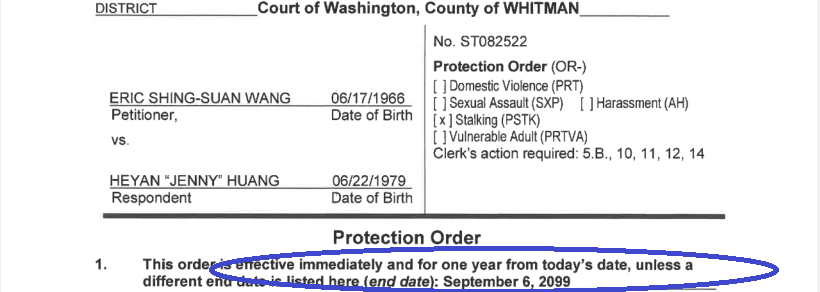
\includegraphics[width=.9\linewidth]{./pic/dearCousin_20220919_222725.png}
\begin{itemize}
\item With about 8-10 more years mature, this slow grown up naive female is finally able to digest necessary concepts with the court and judge as well as launguage interpreter's help. And with a few court hearing dates setup and language interpreter's help, I were able to understand and setup the necessary boundaries, and I learned what I could NOT behave towards Mr. Eric Shing-suan Wang when I have been warned NOT to do.
\item I visited WSU campus during Sep 5 long week end, and had stayed in town for more than 3 business days in hotel. I practiced and succeeded that I have NOT done anything wrong behaviorly toward this magical person Mr. Eric Shing-suan Wang during this vist, till the end of his protection order hearing and safely smoothly left the town for CA.
\end{itemize}

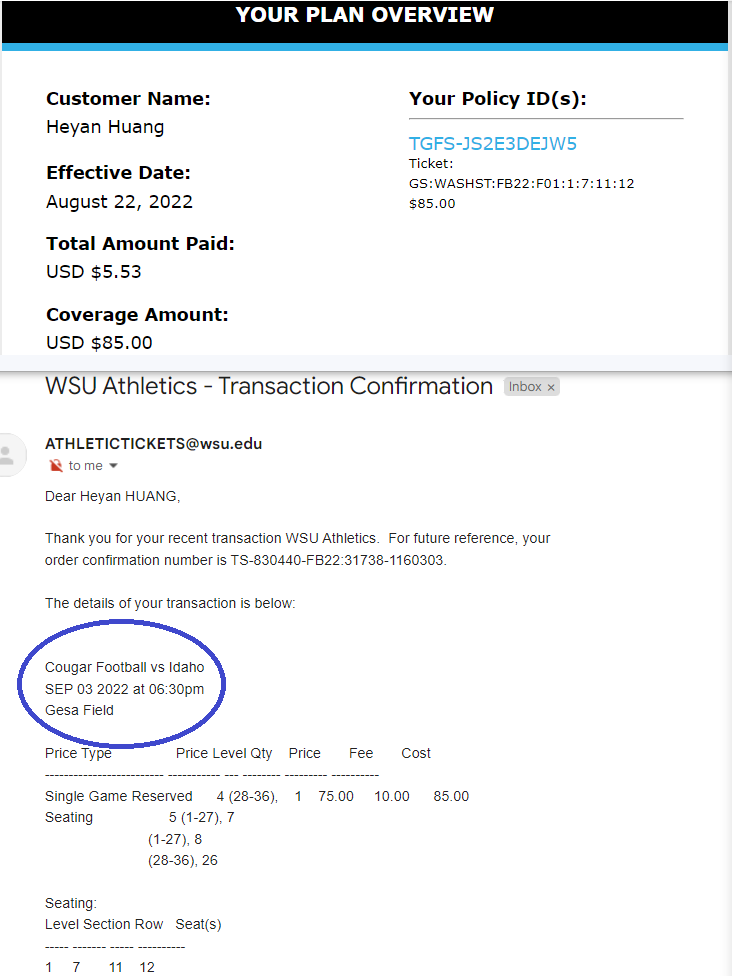
\includegraphics[width=.9\linewidth]{./pic/dearCousin_20220919_225307.png}
\begin{itemize}
\item There is a famous WSU home game this weekend on 9/24/2022, which game I booked ticket for, and I will practice one more and a few more times (later this football game season in Oct. as well as Nov. 2022) to make sure that I learn and grow from this matter.
\end{itemize}

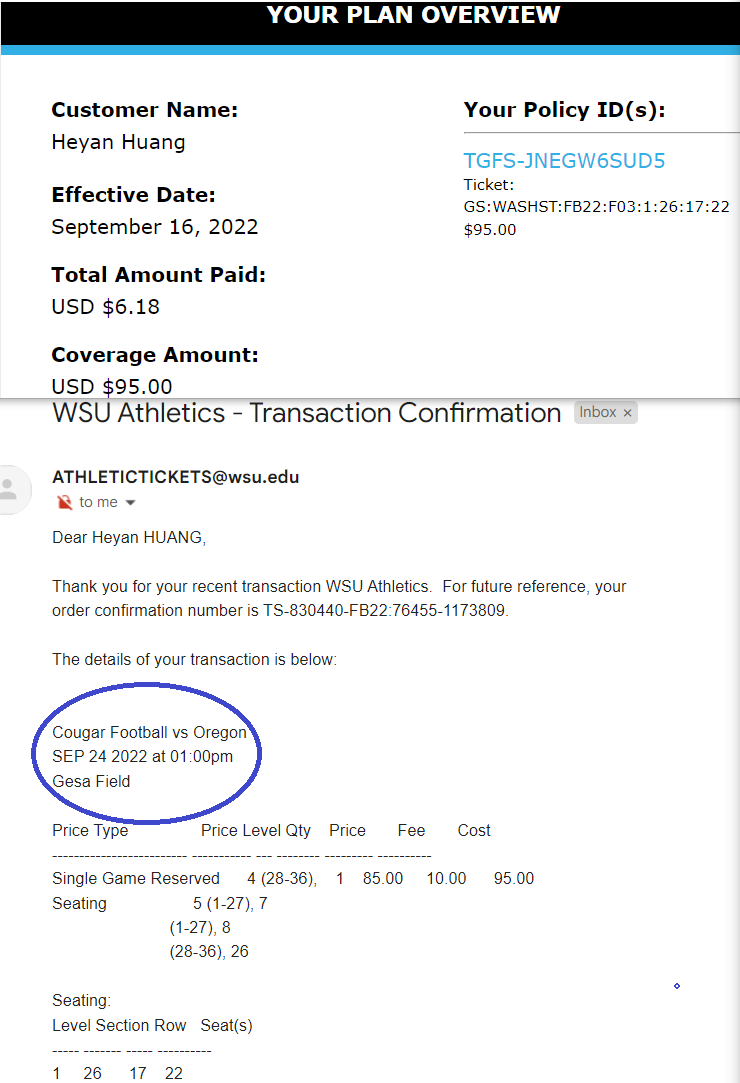
\includegraphics[width=.9\linewidth]{./pic/dearCousin_20220919_221744.png}
\section{个人的认知层面的问题  }
\label{sec-6}
\begin{itemize}
\item 法律是有期限的:所有的限制令都有过期的期限
\end{itemize}
\section{保护令下达(被小地方的法官一羊判便判成了一辈子--至2099呆槑槑槑槑 呵呵)后}
\label{sec-7}
\begin{itemize}
\item If you do not go to court, the judge can make the restraining order without hearing your side of the story. And the order can last up to 5 years.别人也就最多五年,他一弄就弄成了一辈子\url{https://www.courts.ca.gov/1279.htm?rdeLocaleAttr=en}
\item 原令保护令者,可是撒销保护令: The adverse party can file a Motion to Dissolve the protection order, and the court might schedule a hearing on the motion. The applicant can appear at the hearing to oppose the adverse party’s motion. If the Motion to Dissolve is granted after a hearing, the protection order will become immediately void and unenforceable.
\item 我可以appeal反保护令: The adverse party can file a Motion to Modify the protection order, and the court might schedule a hearing on the motion.
\item If an extended protection order is issued, the adverse party can file an appeal to the district court, and the district court might affirm, modify, or vacate the order. The extended protection order remains in effect during any appeal, unless the court orders otherwise.
\end{itemize}
\subsection{Appeal: \url{https://www.civillawselfhelpcenter.org/self-help/harassment-protection/modifying-dissolving-or-appealing-a-protection-order}}
\label{sec-7-1}
\begin{itemize}
\item What is an “appeal,” and how would I file one?
\begin{itemize}
\item If the court issues an extended order for protection, the adverse party can file an appeal to the district court. (There is no appeal allowed if the court denies an application to extend a protection order, only if the court grants the extension.) The district court will typically not hear new evidence on an appeal. The court will review the documentation and other information that was presented to the justice court in order to decide whether the justice of the peace made any error of law in granting the extended protection order.
\end{itemize}
\item The district court can affirm, modify, or vacate the justice court’s order. (In other words, the district court can keep the order in place, change it in some way, or do away with it completely.)
\item TIP!  If the hearing on the extended protection order you're appealing was recorded, you must order a copy of the hearing transcript from the court reporter and deposit \$100 with the court (unless some greater amount was ordered).  (JCRCP 74(b).)  If the hearing wasn't recorded, you must fill out and file the Statement of Evidence or Proceedings form below.
\end{itemize}

\section{几个主要的关注点:根据表哥的陈述,每条反驳回去}
\label{sec-8}
\begin{itemize}
\item to be summarized and finished this evening
\end{itemize}


\section{Statements}
\label{sec-9}
\begin{itemize}
\item 现在的问题是我需要把文件也传给表哥吗?可是我只有一两天的时间[不用再担心这个问题,该发出去的邮件,该寄出去的材料全都寄出去了,最慢也三天之内可以到达了,不用担心]
\end{itemize}
-另外,法庭上还有哪些文件是需要我复制或是转达的吗{暂时也不骼担心这个问题,先把明天傍晚5点前需要上交的材料准备好,交上去,并同步发送给亲爱的表哥就可以了}
-我是否需要立即写封邮件问一下相关的工作人员{已经打电话问好了,就不要再担心了}
\section{oncline resources/ concepts diferences}
\label{sec-10}
\subsection{harassment vs Stalking}
\label{sec-10-1}
-“Harassment” occurs when:
\begin{itemize}
\item The adverse party threatens to harm another person in the future, damages another person’s property, confines or restrains another person, or does any act intended to substantially harm another person’s physical or mental health or safety; AND
\item The adverse party’s words or conduct causes the applicant to reasonably fear that the threats will be carried out.  (NRS 200.571.)
\item “Stalking” occurs when: 
\begin{itemize}
\item The adverse party engages in a course of conduct that would cause a reasonable person to feel terrorized, frightened, intimidated, or harassed or fearful for the immediate safety of a family or household member, AND
\end{itemize}
\end{itemize}
The applicant actually feels terrorized, frightened, or intimidated or fearful for the immediate safety of a family or household member.  (NRS 200.575(1).)
% Emacs 27.1 (Org mode 8.2.7c)
\end{document}